\documentclass{article}
\title{SafeStreets DD}
\date{release date: \today\\version 1}
\author{Matteo Secco, Mohammad Rahbari}
\usepackage{enumitem}
\usepackage{siunitx}
\usepackage{float}
\usepackage{graphicx}
\usepackage[margin=2.5cm]{geometry}
\usepackage{color}
\usepackage[dvipsnames]{xcolor}
\usepackage{listings}
\usepackage{subcaption}
\usepackage{hyperref}
\usepackage{multirow}
\usepackage{tabularx}
\newcommand{\enum}[1]{\texttt{#1.\arabic*}}
\newcommand{\link}[2]{{\color{blue}\underline{\href{#1}{#2}}}}
\begin{document}
\pagenumbering{gobble}
\maketitle
\newpage
\tableofcontents
\pagebreak
\pagenumbering{arabic}


\section{Introduction}

	\subsection{Purpose}
	
		\paragraph{}The required system, called SafeStreets, is a distributed system to allow the citizens to signal parking violations to the competent autorities.
		\paragraph{}The system must allow the citizen to submit pictures of the violation, attaching data such as date, time and position. The user will have to specify the type of the violation when sending these data. 
		\paragraph{}When reciving such data, the system must store them, toghether with the plate of the car that performed the violation (elictated from the picture the citizen sent), the informations about the violation itself (in particular the type of violation), and the name of the street where the violation occourred (which can be retrieved by the positioning information the user sent).
		\paragraph{}In addition, the application must allow both autorities and citizens to analyze the stored data, for example highlighting streets or plates with most violations registered. Different levels of security can be offered.
		\paragraph{}Finally, the application must be enable authorities to automatically generate traffic tickets using its data for people commiting violations, if and only if it can be verified that the data concerning it has not been altered. In this case, SafeStreets could use this informations to build additional statistics.

		\subsubsection{Goal list}
			\begin{enumerate}[label=\enum{G}]
				\item  \label{G:realTime}Allow citizens to notify parking violations and be acknowledged of the result as soon as possible
				\item \label{G:allData}Force citizens to provide all the needed data about violation, in particular infraction type, picture, date, time and position
				\item \label{G:helpAuth}Prevent the autorities to have to manually address parking tickets
				\item \label{G:discardAltered} Ensure no tickets can be emitted if the notification's data has been modified somehow
				\item \label{G:respectPermissions} Ensure no tickets can be emitted if the plate of the car that committed the infringment owns a permission for that infringiment
				\item \label{G:storeFine} Every notification not covered by \ref{G:discardAltered} or \ref{G:respectPermissions} will be eligible for ticket generation
				\item \label{G:statistics}Allow both citizens and authorities retrive informations about previous violations and released tickets, possibly in an aggregated form. Every violation reported to the system and stored will appear in some statistics
				
			\end{enumerate}

	\subsection{Scope} 
	The world where the system must fit is an everday city, with focus on the traffic of moterized veichles.\\
	The events the system aims to influence are the parking of motorized veichles,  in particular the ones considered infractions.\\
	In the context of the system, when any user notices an illegal parking, he/she may notify the system and provide any needed informations to the competent authorities. In particular, the notification is composed by a picture of the infraction, a timestamp (date and time), the geographical location of the infraction and the type of infraction wich is to be notified. Some of these informations can be gathered automatically from the user's device. Notice that, for legal reasons, SafeStreets will just make the data available to the auth, and will \underline{not} generate tickets itself. \\
	In addiction, the user may interrogate the system to gather aggregated informations about the locations with more violation incidence, and the cars which committed more violations. 
	
	\begin{table}[H]
	\begin{center}
		\caption{Phenomena}
		\small
		\begin{tabular}{|l|c|c|}
			\hline
			\textbf{Phenomenon}		&	\textbf{Shared}&\textbf{Who controls it}\\
			\hline
			A citizen parks its car	&	N	&	W\\
			A citizen spots a car in 
			an illegal parking		&	N	&	W\\
			A citizen wants to
			notify a violation		&	Y	&	W\\
			The user fills the data
			needed to notify 
			a violation				&	Y	&	W\\
			The machine revices a
			notification, analyzes
			it and stored stores it 
			if it's trusted			&	N	&	M\\
			A user requests
			map statistics			&	Y	&	W\\
			A citizen requests
			top violators statistics	&	Y	&	W\\
			The machine analyzes
			data and builds 
			statistics				&	N	&	M\\
			Statistics are organized
			and presented
			to the user				&	Y	&	M\\
			An authority wants to
			generate tickets			&	N	&	W\\
			An authority requests
			some violation notified
			and stored in the
			machine					&	Y	&	W\\
			The machine provides
			some notification to
			an authority requesting
			them						&	Y	&	M\\
			The authority decides
			whether generate a ticket
			for a violation or not	&	Y	&	W\\
			The authority generates
			a ticket for a
			violation				&	N	&	W\\
			The authority informs
			the machine she has 
			generated a ticket 
			for a given violation	&	Y	&	W\\
			An authority requests
			informative statistics
			about its competence 
			area						&	Y	&	W\\
			\hline
		\end{tabular}				
	\end{center}
	\end{table}
		
	\subsection{Definitions, Acronyms,Abbreviations} \label{definitions}
		\paragraph{Person:}A person in the real world. Every Citizen is a person, generally an Authorithy is not
		\paragraph{User:}A person, an organization or a system which somehow uses SafeStreets
		\paragraph{Citizen (cit):} This term will be used to denote every \underline{user} not owning particular privileges or permissions. A citizen is only allowed to notify violations and see some aggregated data
		\paragraph{Authority (auth):} This term will denote every \underline{user} (phisical or digital) having privileged access to the stored data. An example of Authority is the Local Police.
		\paragraph{Notification:} 
			\begin{list}{-}{Represents a set of data submitted by any user composed by:}
				\item A picture of a parking infraction
				\item A timestamp of when the notification occourred, containing date and time (may be gathered automatically by the citizen's device)
				\item A geographical position of where the infraction occurred (may be gathered automatically by the citizen's device)
				\item The type of infraction notified
			\end{list}
		\paragraph{Car:}The word car will be used to issue every mothorized vehicle
		\paragraph{Plate:}Identifies a \underline{car}
		\paragraph{Permisison:}A document released by a verified authority, granting to a car the permission to park in a set of reserved parkings (ex: permission to park on parking reserved for disabled people). 
		
	\subsection{Revision history}
	\subsection{Reference documents}
	\subsection{Document Structure}

\section{Architectural Design}
	\subsection{Overview} \textit{High-level components and their interaction}
	In this section the architectural design of SafeStreets is presented. 
	\begin{list}{$\bullet$}{The presentation is divided into the following parts:}
		\item \textbf{High level architecture:} 
			This section will provide an high level view of the system architecture.
		\item \textbf{Data model:}
			This part will describe the Database structure.
		\item \textbf{Component view:} 
			This part will introduce all the components the system will be made from, their functionalities and their interactions.
		\item \textbf{Deployment view:} 
			This part describes the hardware that will compose the system as well as the software that will be runned on it.
		\item \textbf{Runtime view:} 
			This parts describes in detail the executon behaviour of each component.
		\item \textbf{Component interfaces:} 
			This pat describes the interface that the components will use to communicate one with the other, as well as the interfaces with other
			systems.
		\item \textbf{Selected architectural styles and patterns:} 
			This parts describes the design choices  about the architecture of the application.
	\end{list}
	\subsection{High level architecture}
	\subsection{Data model} The data will be stored in a cloud-based relational database. The following Entity-Relationship diagram explains which data the system will store and manage
	\begin{figure}[H]
		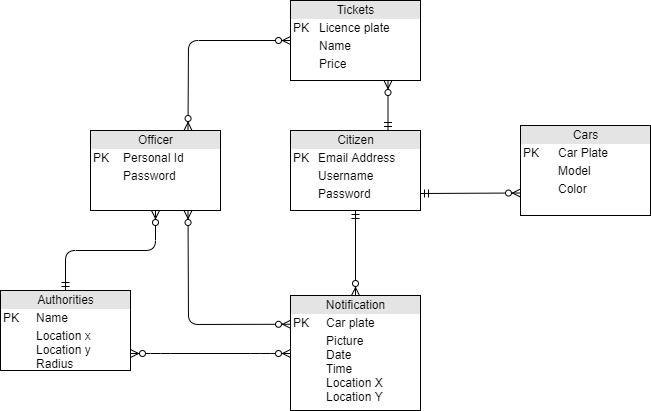
\includegraphics[width=\linewidth]{images/Data_model_diagram.png}
		\caption{Data model diagram}
	\end{figure}
	\subsection{Component view} \label{Section:Component view} \textit{Here we thescribe how the project can be modularized}\\
	\begin{figure}
		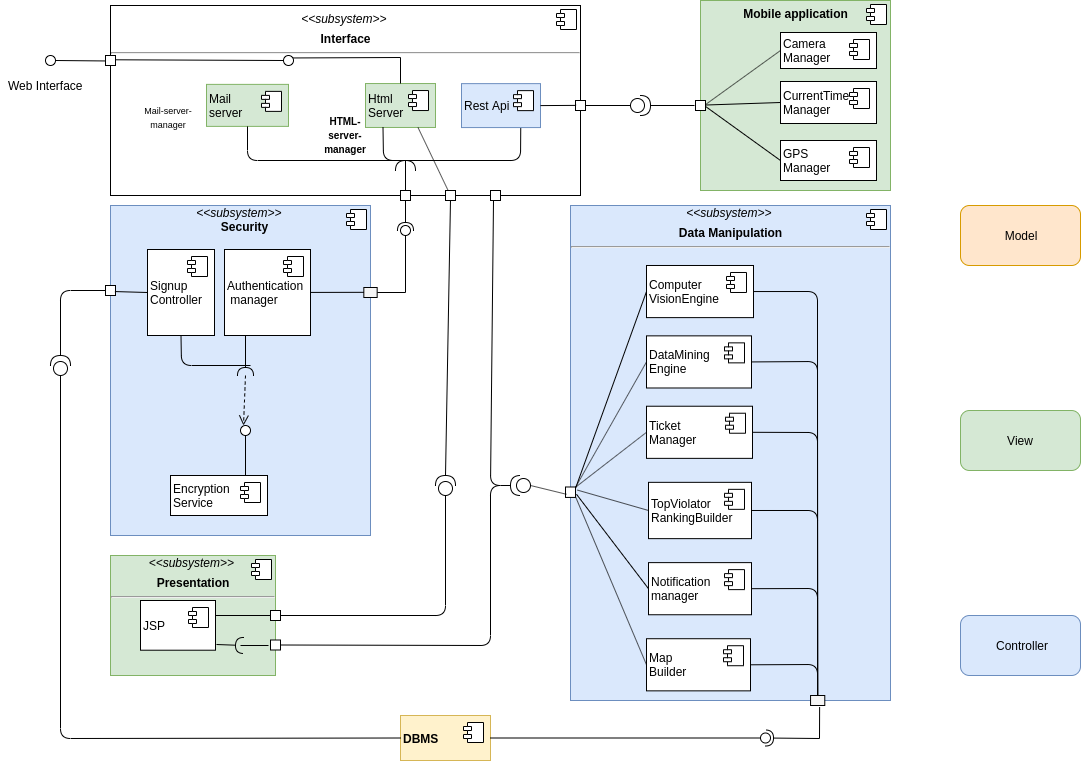
\includegraphics[width=\linewidth]{images/Component_Diagram.png}
		\caption{Component Diagram (Client components are omitted for brevity)}
	\end{figure}
	The following table collects the component by functional group and by user group:
	\begin{table}[H]
	\begin{center}
		\caption{Components}
		\small
		\begin{tabular}{|l|l|l|l|l|l|}
		\hline
		&\textbf{Security}			&\textbf{Interfaces}	&\textbf{Presentation}		&\textbf{Data manipulation}	&\textbf{Storage}\\
		\hline
		\textbf{Server}	
		&AuthenticationManager		&HtmlServer			&NotificationManager			&ComputerVisionEngine		&	DBMS\\
		&SignupController			&MailServer			&MapBuilder					&DataMiningEngine			&		\\
		&EncryptionService			&RestApi		&TopViolatorsRankingBuilder	&TicketManager				&		\\
		&							&					&StatisticsPresenter			&							&		\\
		&							&					&TicketPresenter				&							&		\\
		&							&					&JSP							&							&		\\
		\hline
		\textbf{Citizen}
		&EncryptionService			&RestApi		&MapDisplayer				&CameraManager				&		\\
		&							&					&TopViolatorsDisplayer		&GPSManager					&		\\
		&							&					&NotificationService			&CurrentTimeManager			&		\\
		\hline
		\textbf{Authority}
		&							&WebBrowser			&WebBrowser					&							&		\\
		\hline
		\end{tabular}
	\end{center}
	\end{table}
	The following list provides a detailed description of each module's functionalities (calls to components are omitted here as they will be
	datailed in sequence diagrams):
	\begin{itemize}
		\item \label{component:AuthenticationManager} \textbf{AuthenticationManager:}
			This module will authenticate the user comparing the provided credentials with the ones stored to the database, and if a match is found
			will generate a session token for authentication. The provided password will be hashed before comparison (as passwords won't be stored
			in plain text). The usage of a token (nounce) can prevent many malicious attacks, such as 
		 	\link{https://en.wikipedia.org/wiki/Cross-site_request_forgery}{Csrf attacks} or 
			\link{https://en.wikipedia.org/wiki/Replay_attack}{Replay attacks}. 
		 \item \label{component:SignupController} \textbf{SignupController:} 
		 	This component will manage the signup procedure, in particular it's main functionalities will be: reciving a signup request, check the
		 	constraints of the provided data (in example, unicity of username and email, strength of the password), hash the password, temporary store these data, 
		 	generate and send a token to the given email to verify it, persistently store the data. The email validation can provide some protection against
		 	\link{https://en.wikipedia.org/wiki/Denial-of-service_attack}{DoS attacks}, but full protection is
		 	currently unachievable (many researches are running to find a solution)
		 \item \label{component:EncryptionService} \textbf{EncryptionService:}
		 	\link{https://en.wikipedia.org/wiki/Bcrypt}{BCrypt}
		 \item \label{component:HtmlServer} \textbf{HtmlServer:}
		 	This component is an interface to handle \link{https://en.wikipedia.org/wiki/Hypertext_Transfer_Protocol}{http} requests for the HTML pages to be displayed
		 	on a web browser. 
		 \item \label{component:MailServer} \textbf{MailServer:} 
		 	This component is an interface for mail sending emails to the users, in particular notifications (i.e: a ticket has been issued to them) and the first email
		 	used to confirm the email address.
		 \item \label{component:RestApi} \textbf{RestApi:} 
		 	This component will handle the custom messaging protocol with Citizen's devices. The communication will rely on HTTPS, in order to protect the system from 
		 	\link{https://en.wikipedia.org/wiki/Man-in-the-middle_attack}{Man in the Middle attacks}.
		 \item \label{component:JSP} \textbf{\link{https://en.wikipedia.org/wiki/JavaServer_Pages}{JSP:}}
		 	This component, relying on a well-known technology, will dynamically create HTML data starting from given templates and data.
		 \item \label{component:NotificationManager} \textbf{NotificationManager:}
		 	This component will decide when is needed to send a notification to an User, by sending an email in case of Authorities, or by displaying a notification 
		 	on the application and/or sending an email in case of Citizens, according to the preferences they setted.
		 \item \label{component:MapBuilder} \textbf{MapBuilder:}
		 	This component is responsible to aggregate data from the database according to a geographical location, and to create the data needed to display them
		 	using the Google Maps API.
		 \item \label{component:TopViolatorsRankingBuilder} \textbf{TopViolatorsRankingBuilder:}
		 	This component will query the database for Violations based on a geographical location, hide the plate from pictures and
		 	generate the list for the Top Violators page.
		 \item \label{component:ComputerVisionEngine} \textbf{ComponentVisionEngine:}
		 	The main functionality of this component is to recive a picture and extract the car plate out of it.
		 	It will also be used to hide the plates from the TopViolatorsRanking.
		 \item \label{component:DataMiningEngine} \textbf{DataMiningEngine:}
		 	This component will run data mining algorithms on the database to discover relevant informations with regard to specific geographical
		 	locations.
		 \item \label{component:TicketManager} \textbf{TicketManager:}
		 	This component will filter incoming notifications in order to avoid to store non-ticketable violations, and provide stored violations that are
		 	issuable on demand.
		 \item \label{component:CameraManager} \textbf{CameraManager:}
		 	This component will grant secure access to the camera of a Citizen's device, preventing it from notifying violations if the camera is not 
		 	available (for hardware fault or denied permission).
		 \item \label{component:GPSManager} \textbf{GPSManager:}
		 	This component will regulate the access to the GPS of the citizen device, as well as the gathering of the position.
		 \item \label{component:CurrentTimeManager} \textbf{CurrentTimeManager:}
		 	This component will check if the date and time settings on the user device are set to auto (the device synchronizes it's clock using 
		 	internet or the GPS). If they are, the current time is collected, otherwise the notification is blocked until the settings are changed
		 \item \label{component:DBMS} \textbf{DBMS:}
		 	This component will be respopnsible of managing the database.
	\end{itemize}
	\newpage
	\subsection{Deployment view} How the modules are implemented, explaying both hardware and software
	\begin{figure}[H]
		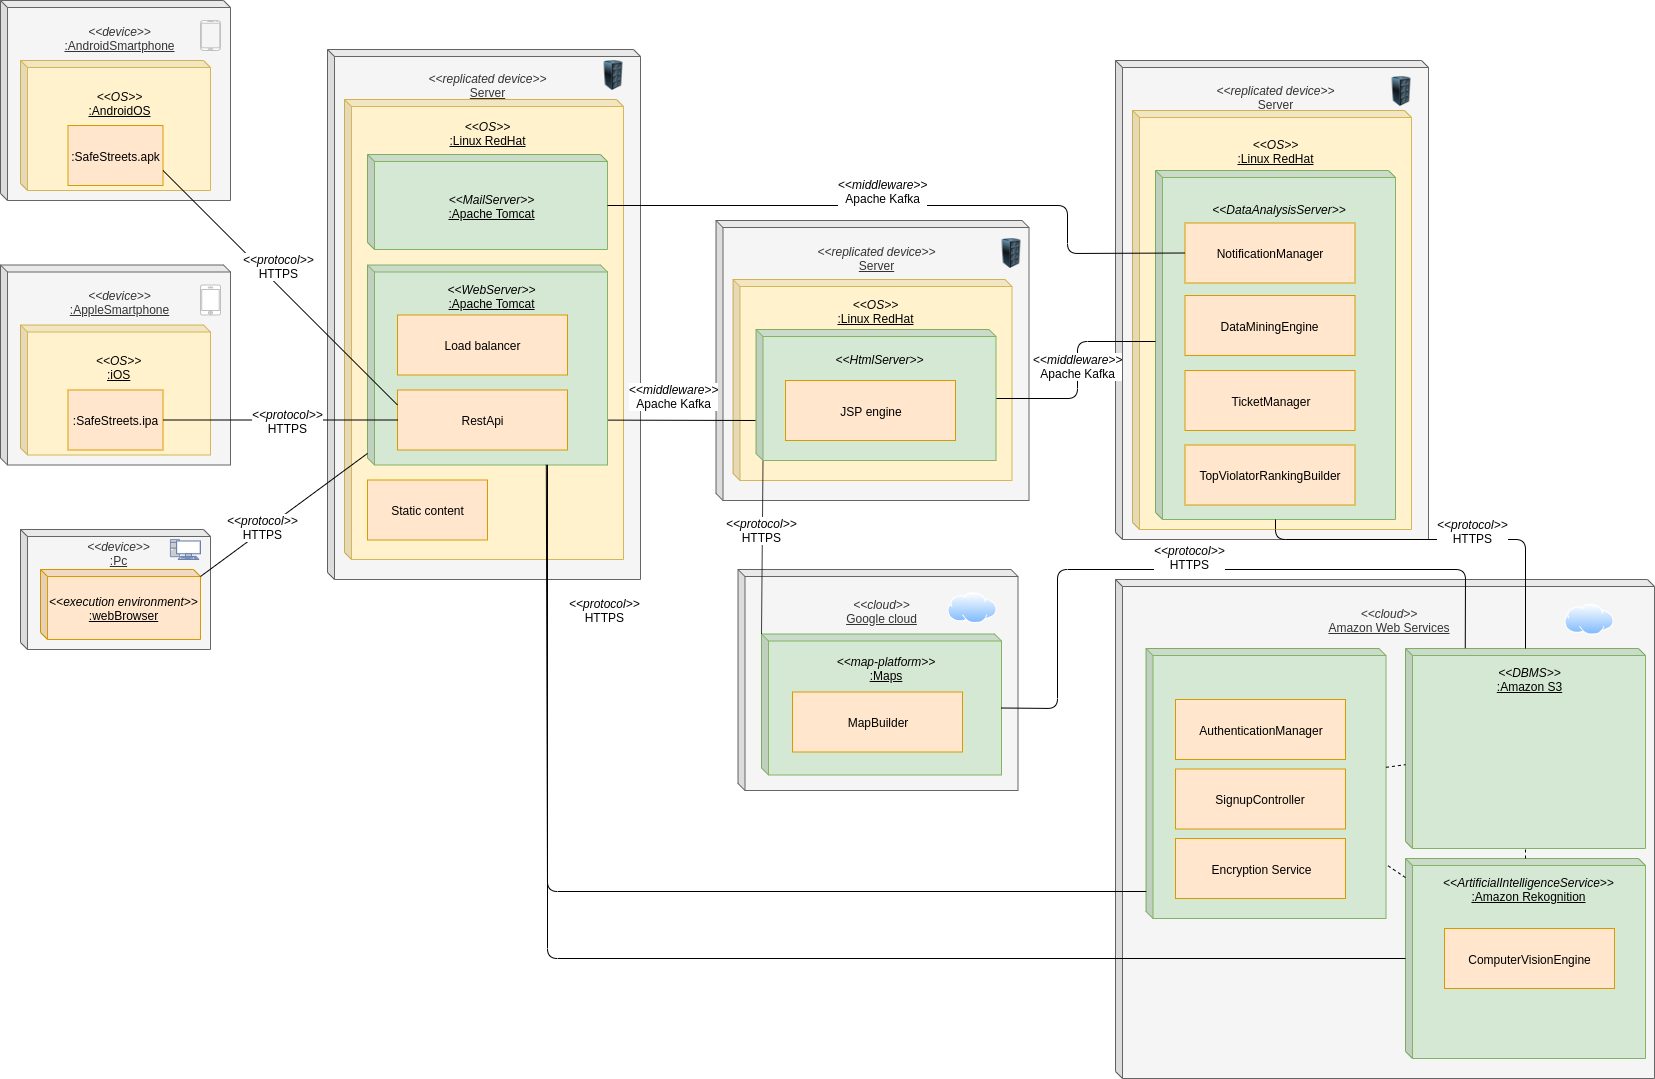
\includegraphics[width=\linewidth]{images/Deployment_diagram.png}
		\caption{Deployment diagram}
	\end{figure}
	\newpage
	\subsection{Runtime view} The following diagrams show the interactions between components in order to achieve the
	required functions
	\begin{figure}[H]
		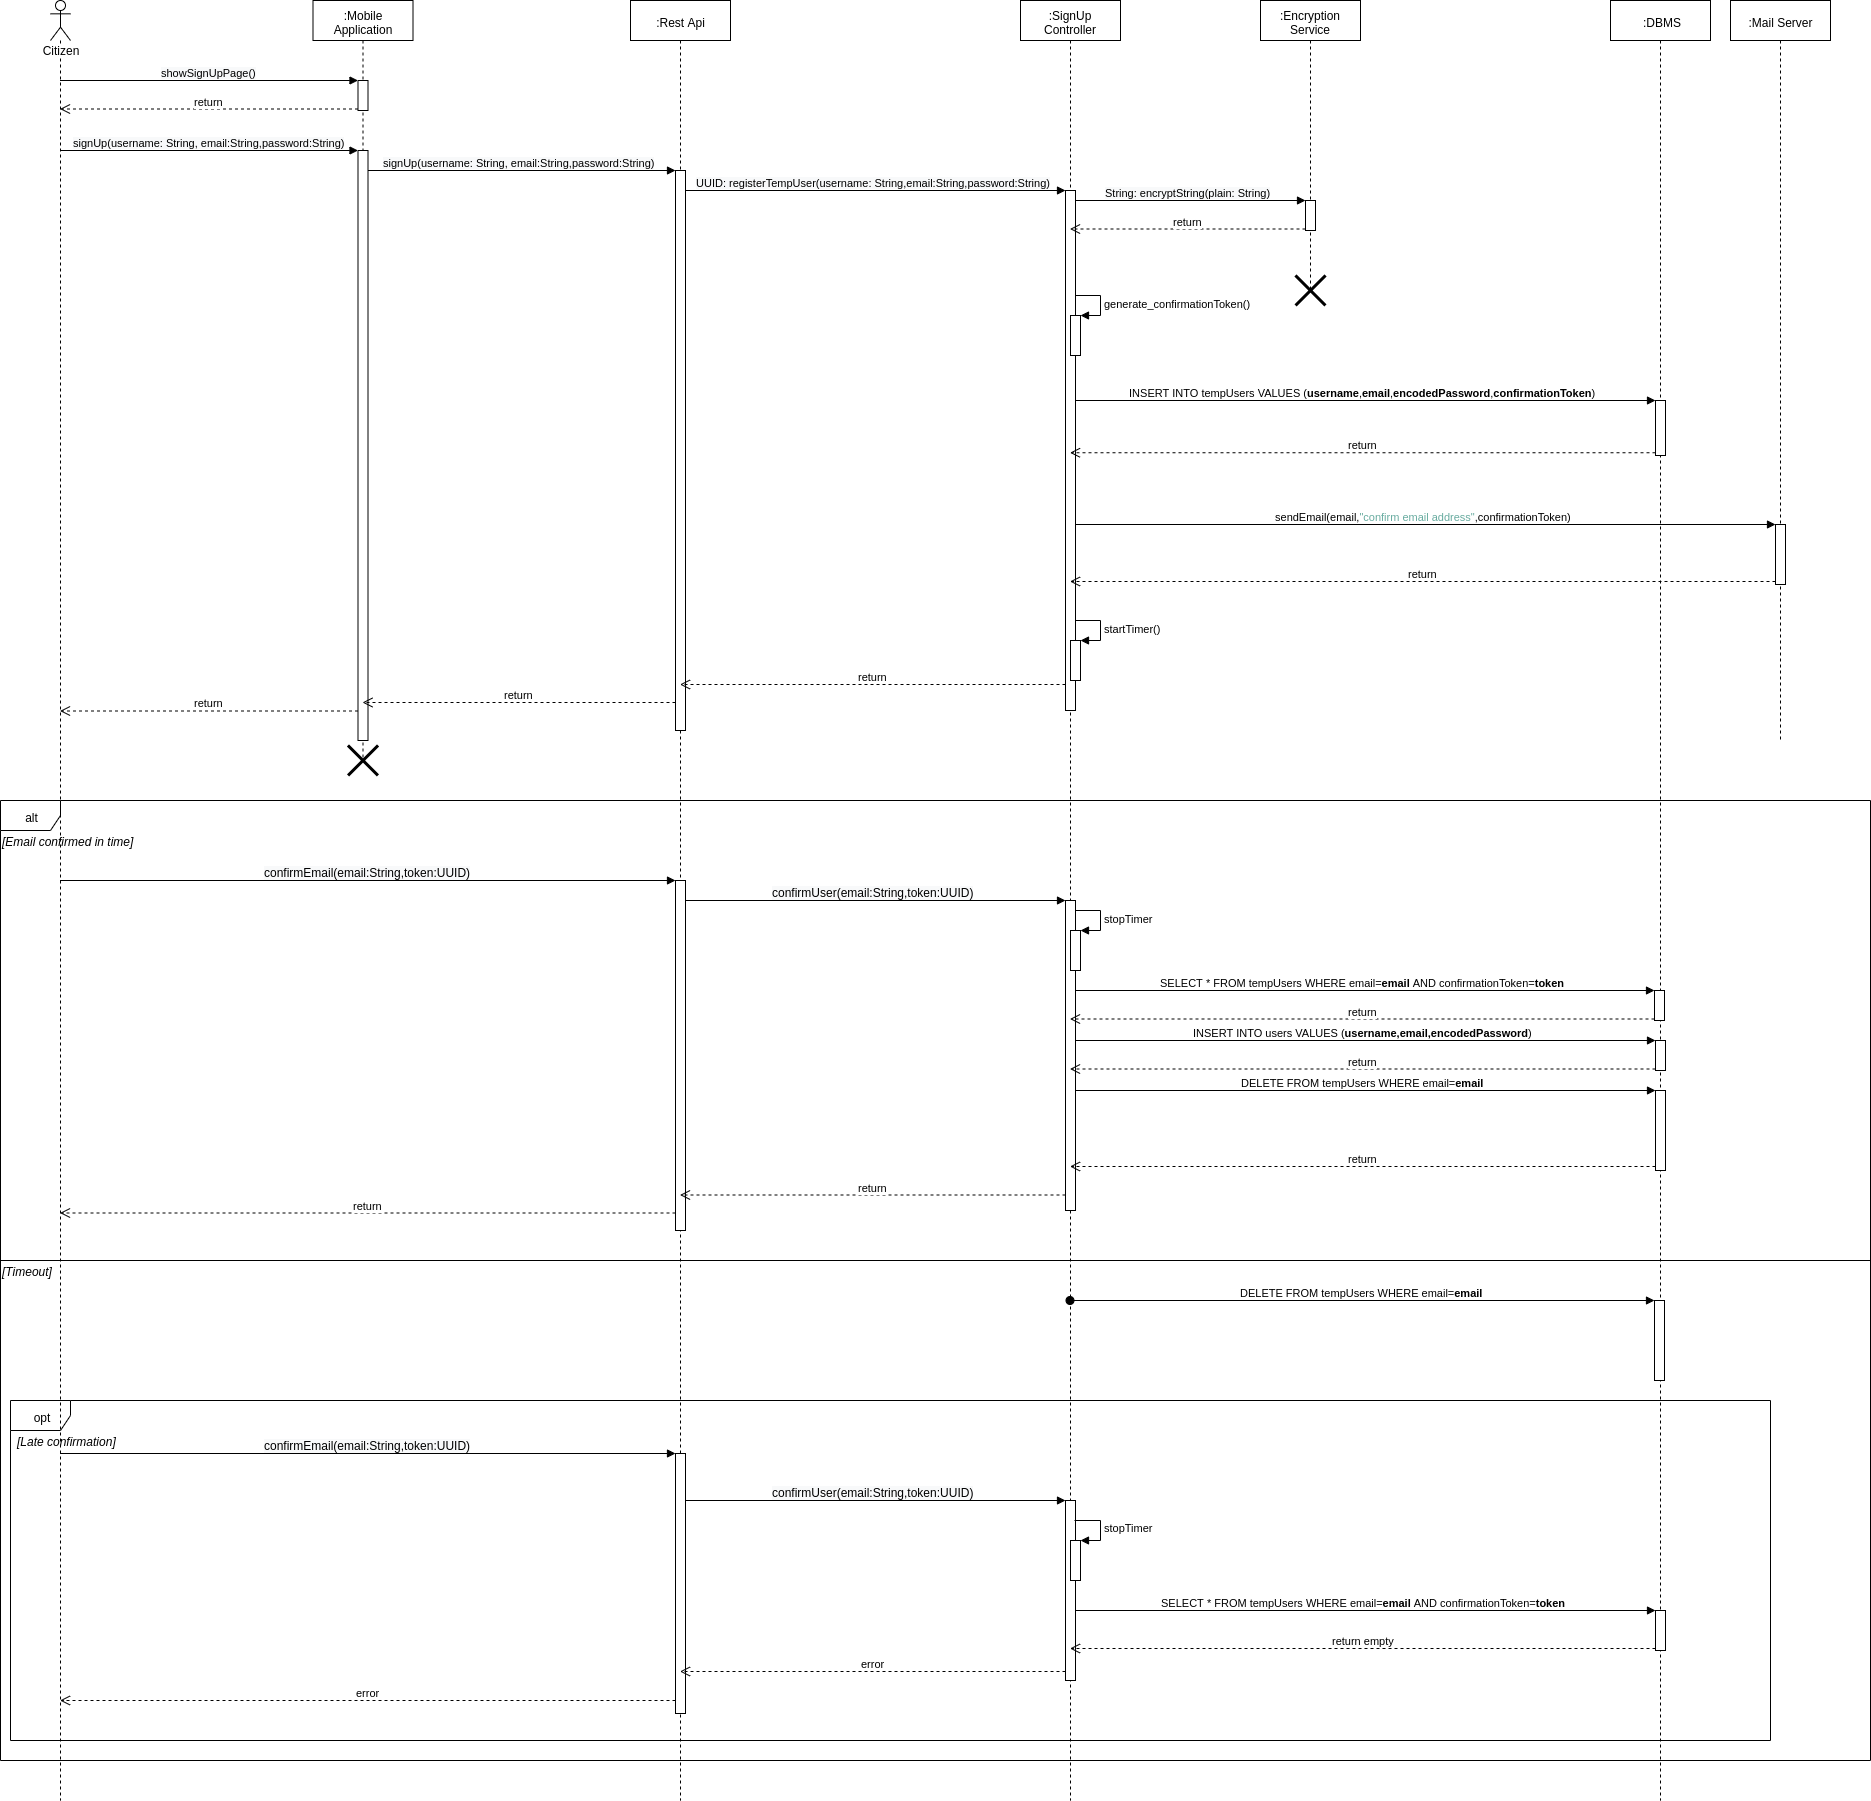
\includegraphics[width=\linewidth]{images/Register_citizen_sequence_diagram.png}
		\caption{Register citizen sequence diagram}
	\end{figure}
	\begin{figure}[H]
		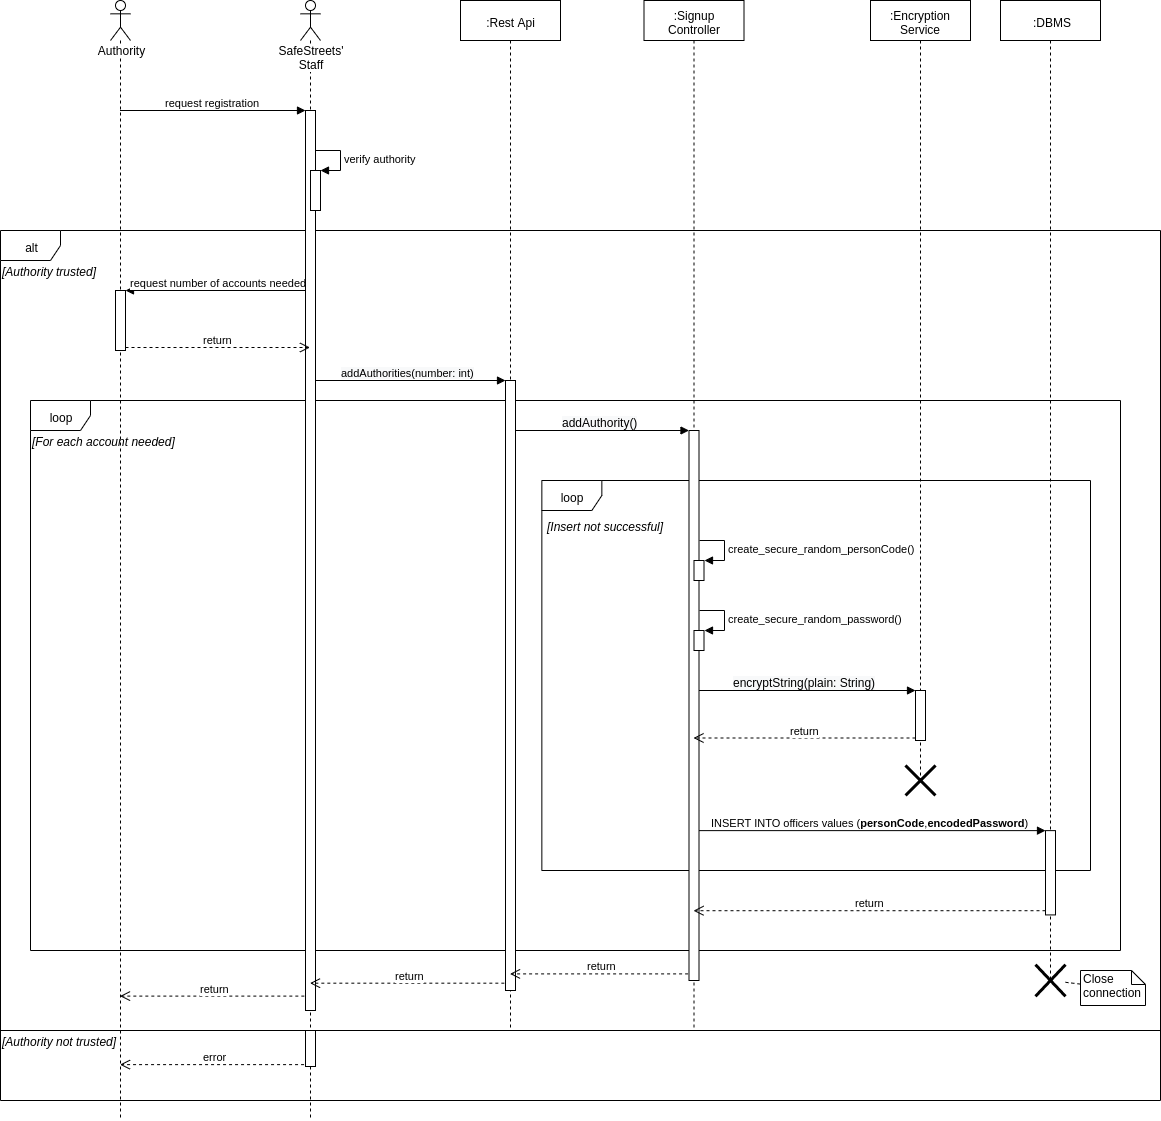
\includegraphics[width=\linewidth]{images/Register_authority_sequence_diagram.png}
		\caption{Register authority sequence diagram}
	\end{figure}
	\begin{figure}[H]
		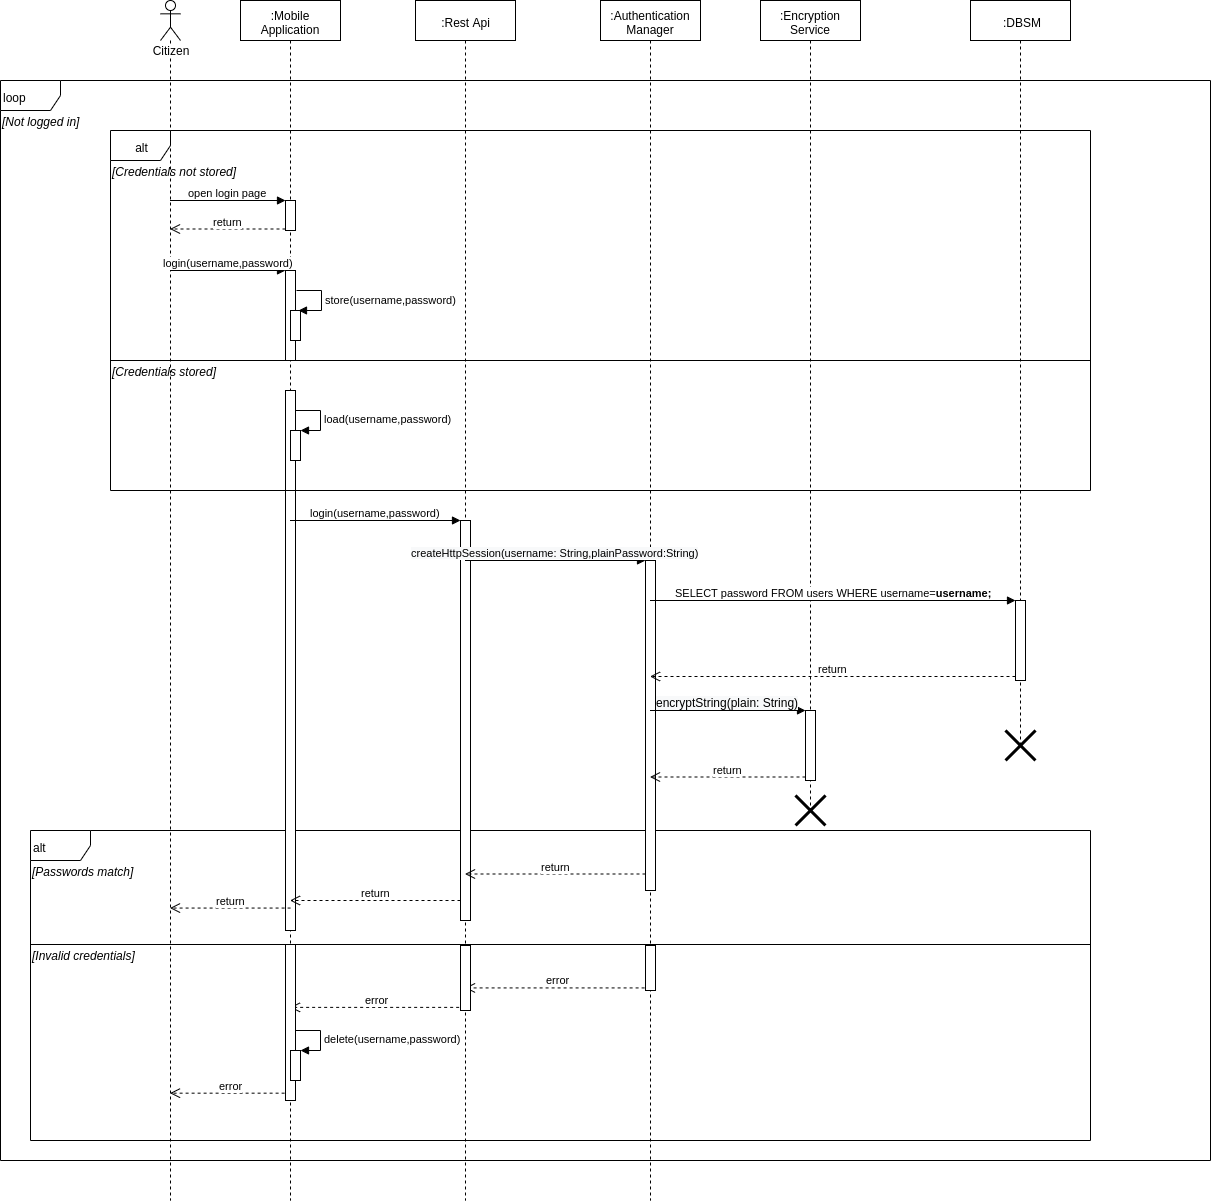
\includegraphics[width=\linewidth]{images/Login(Citizen)_sequence_diagram.png}
		\caption{Login citizen sequence diagram}
	\end{figure}
	\begin{figure}[H]
		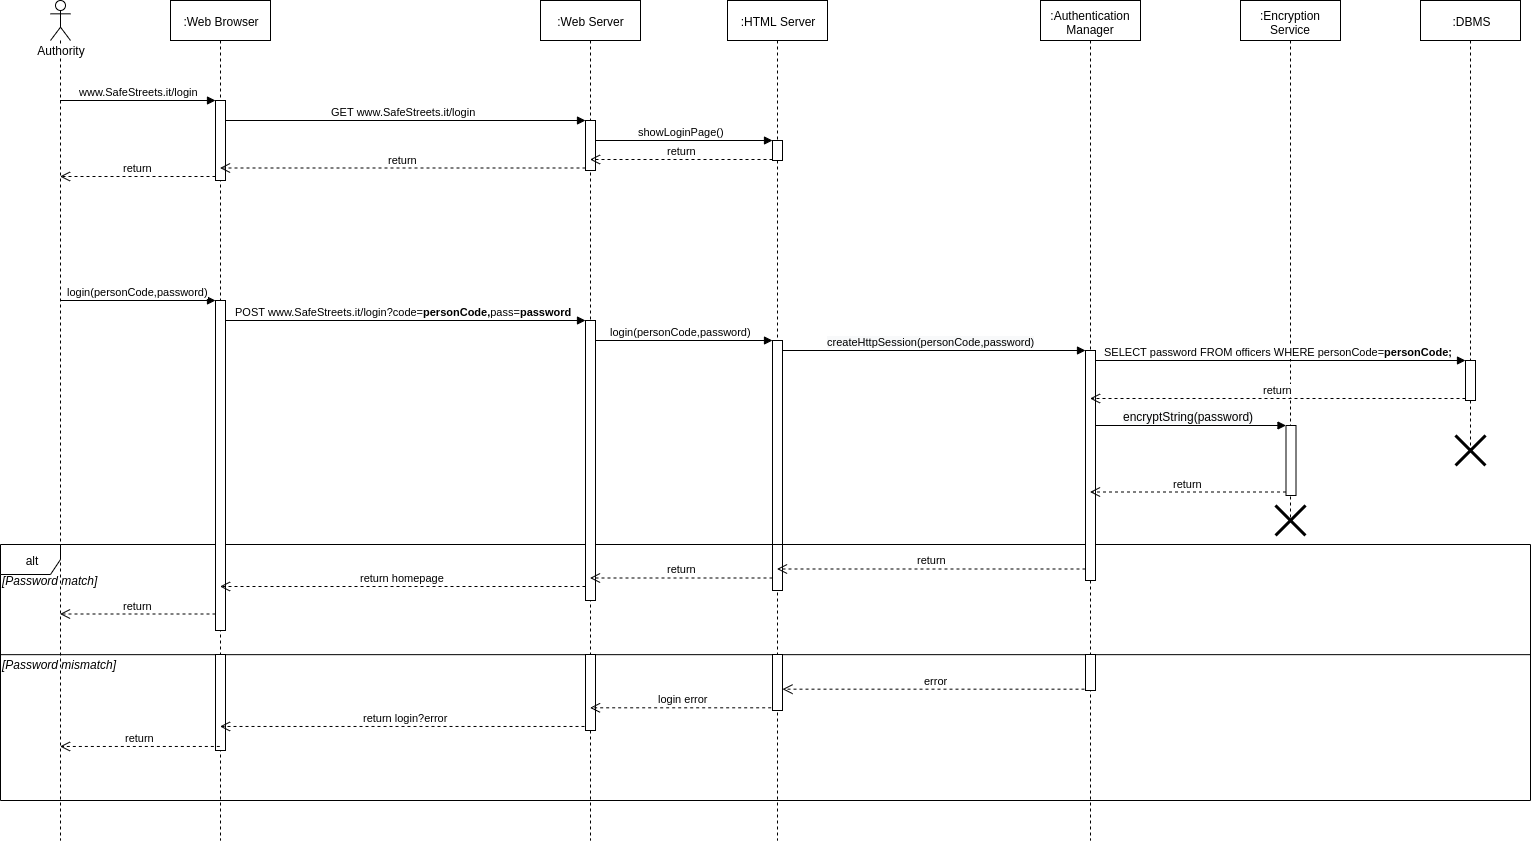
\includegraphics[width=\linewidth]{images/Login(authority)_sequence_diagram.png}
		\caption{Login authority sequence diagram}
	\end{figure}
	
	\begin{figure}[H]
		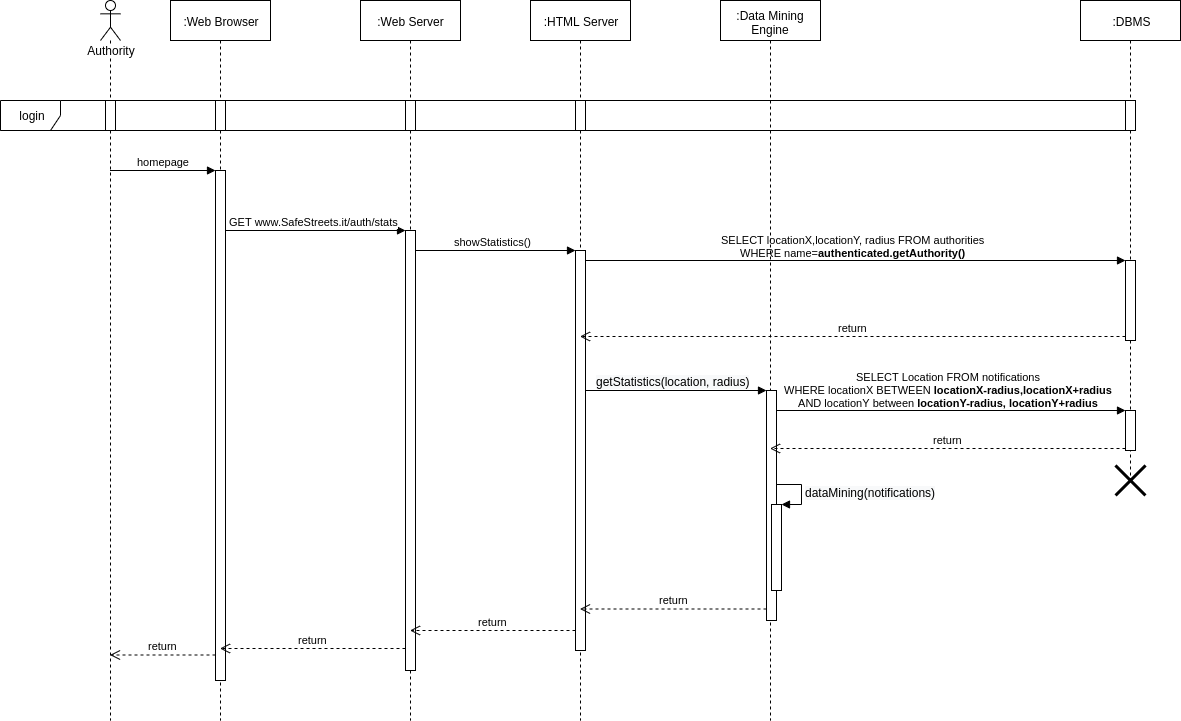
\includegraphics[width=\linewidth]{images/See_statistics_sequence_diagram.png}
		\caption{See statistics sequence diagram}
	\end{figure}
	\begin{figure}[H]
		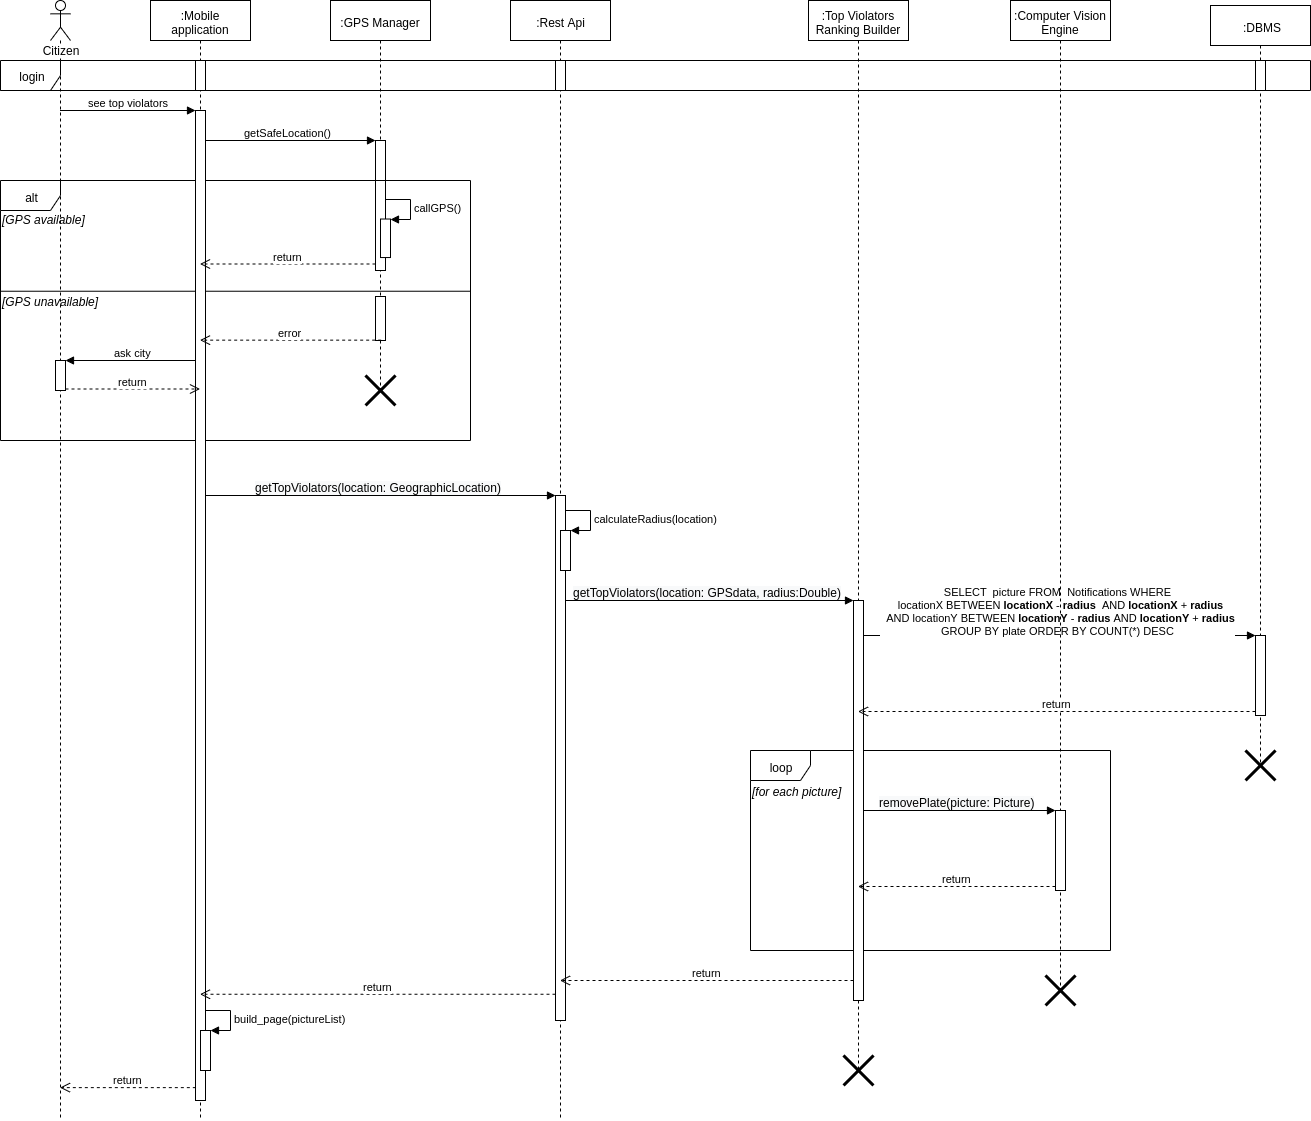
\includegraphics[width=\linewidth]{images/See_Top_Violators_Sequence_Diagram.png}
		\caption{See top violators ranking sequence diagram}
	\end{figure}
	\begin{figure}[H]
		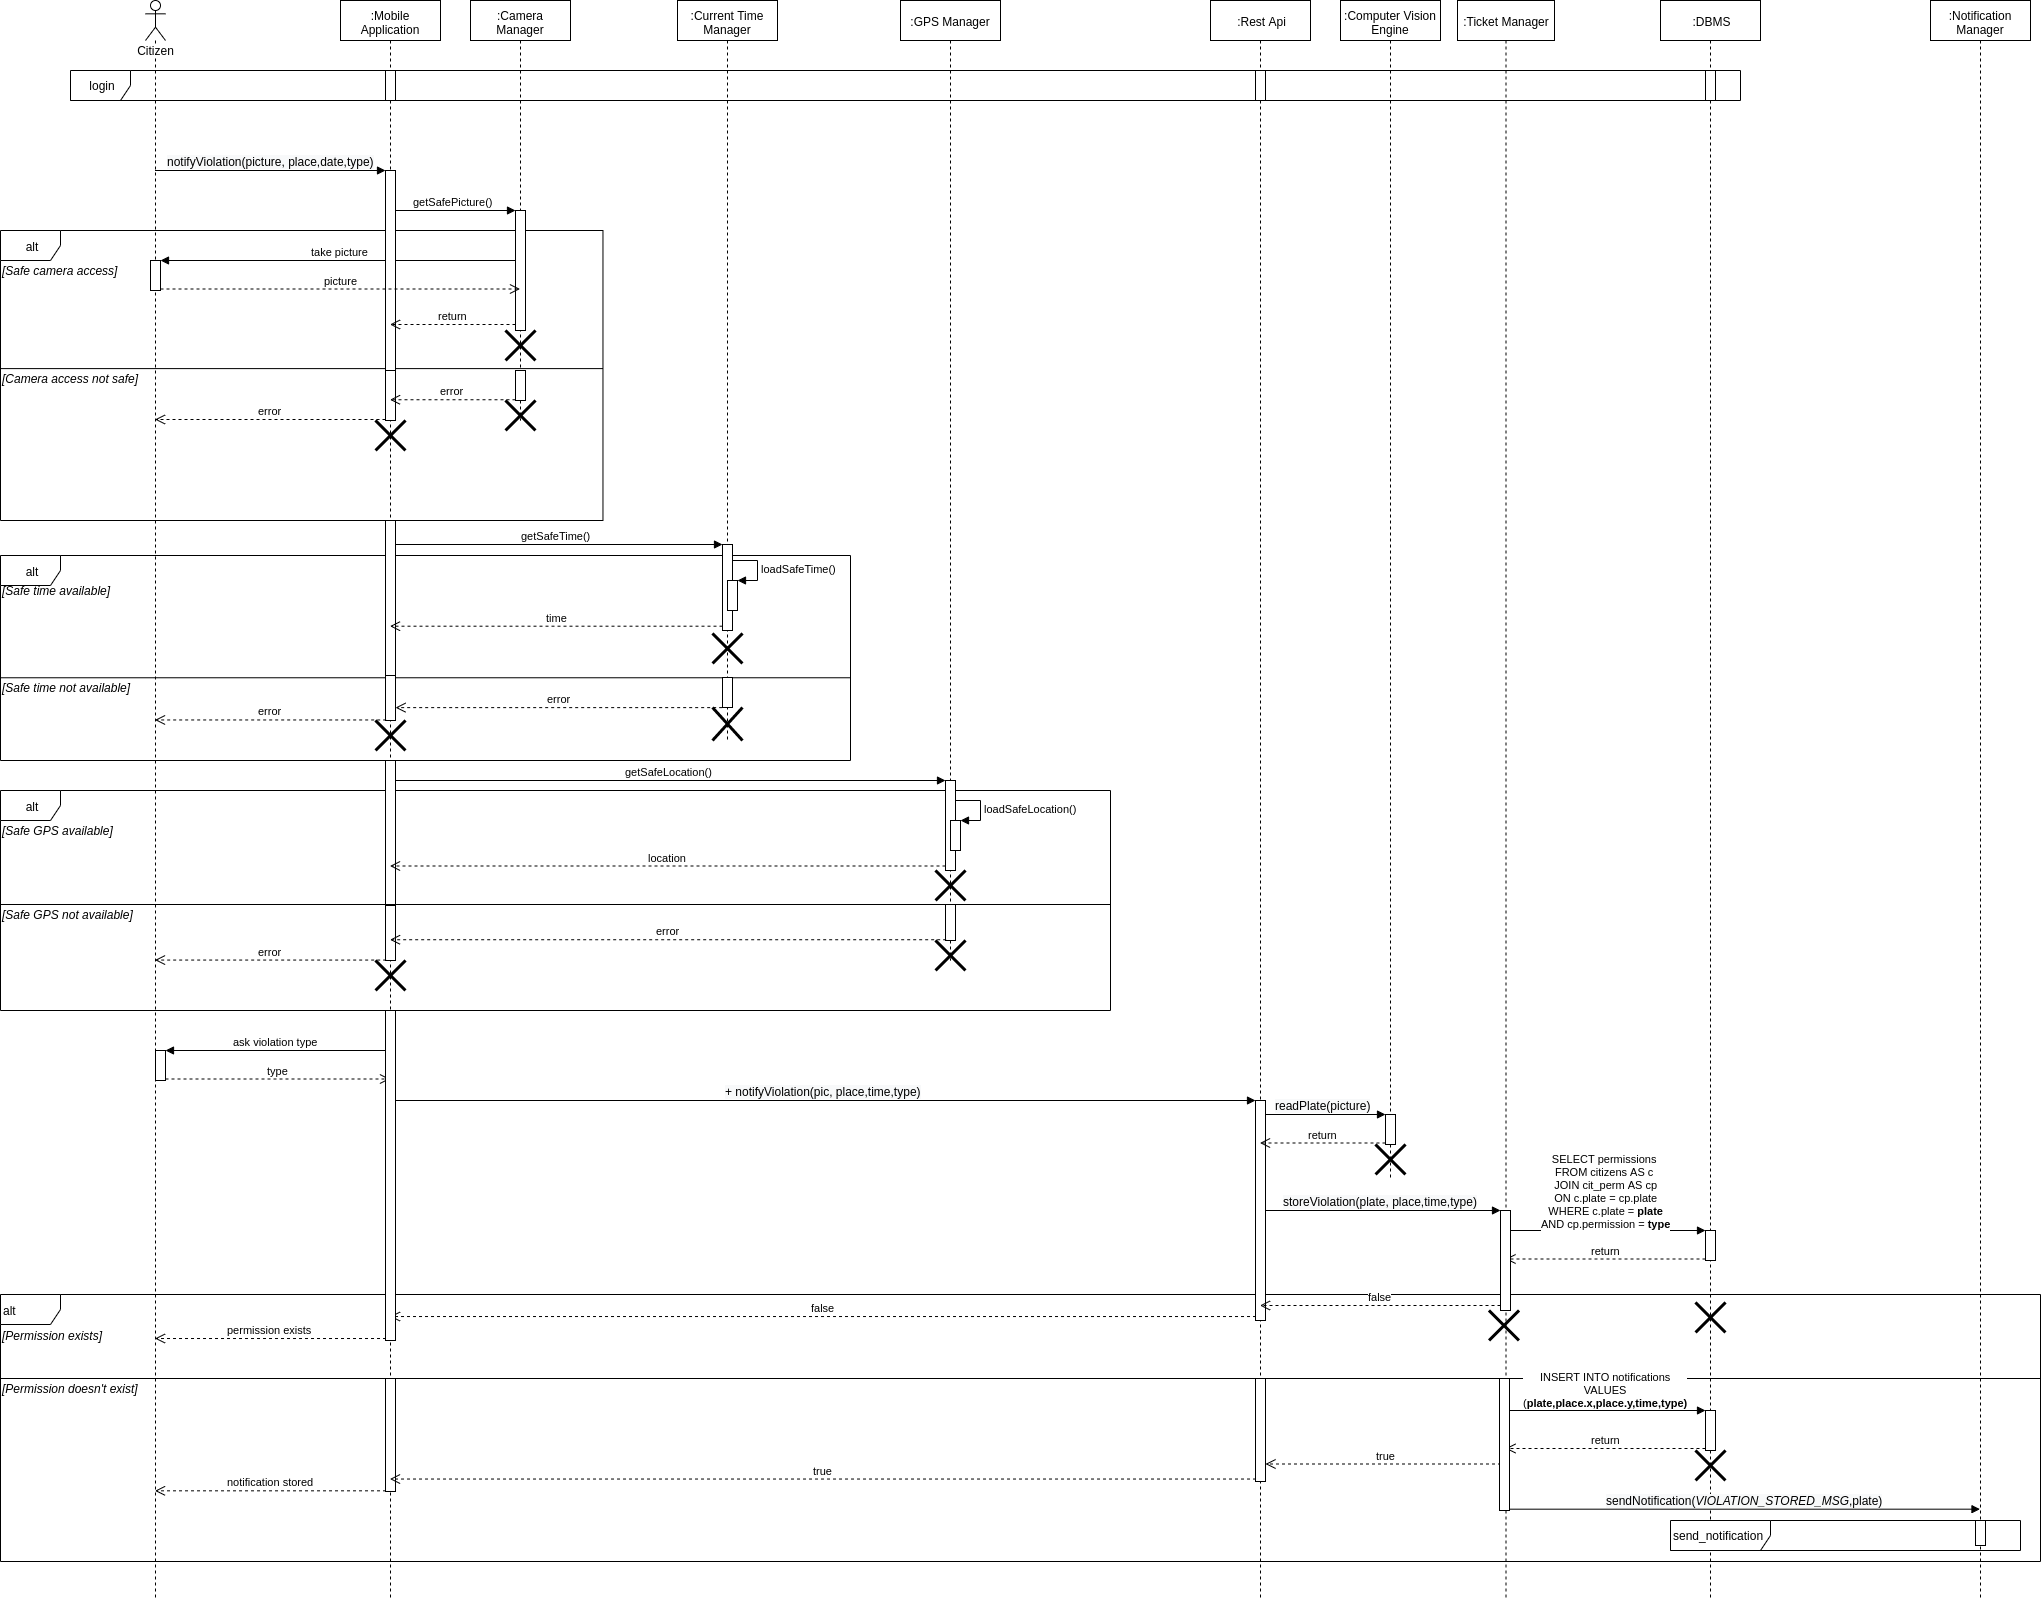
\includegraphics[width=\linewidth]{images/Notify_Violation_sequence_diagram.png}
		\caption{Notify violation sequence diagram}
	\end{figure}
	
	
	\newpage
	\subsection{Component Interfaces}
	The following diagram illustrates the interfaces and the dependencies between different components.
		\begin{figure}[H]
			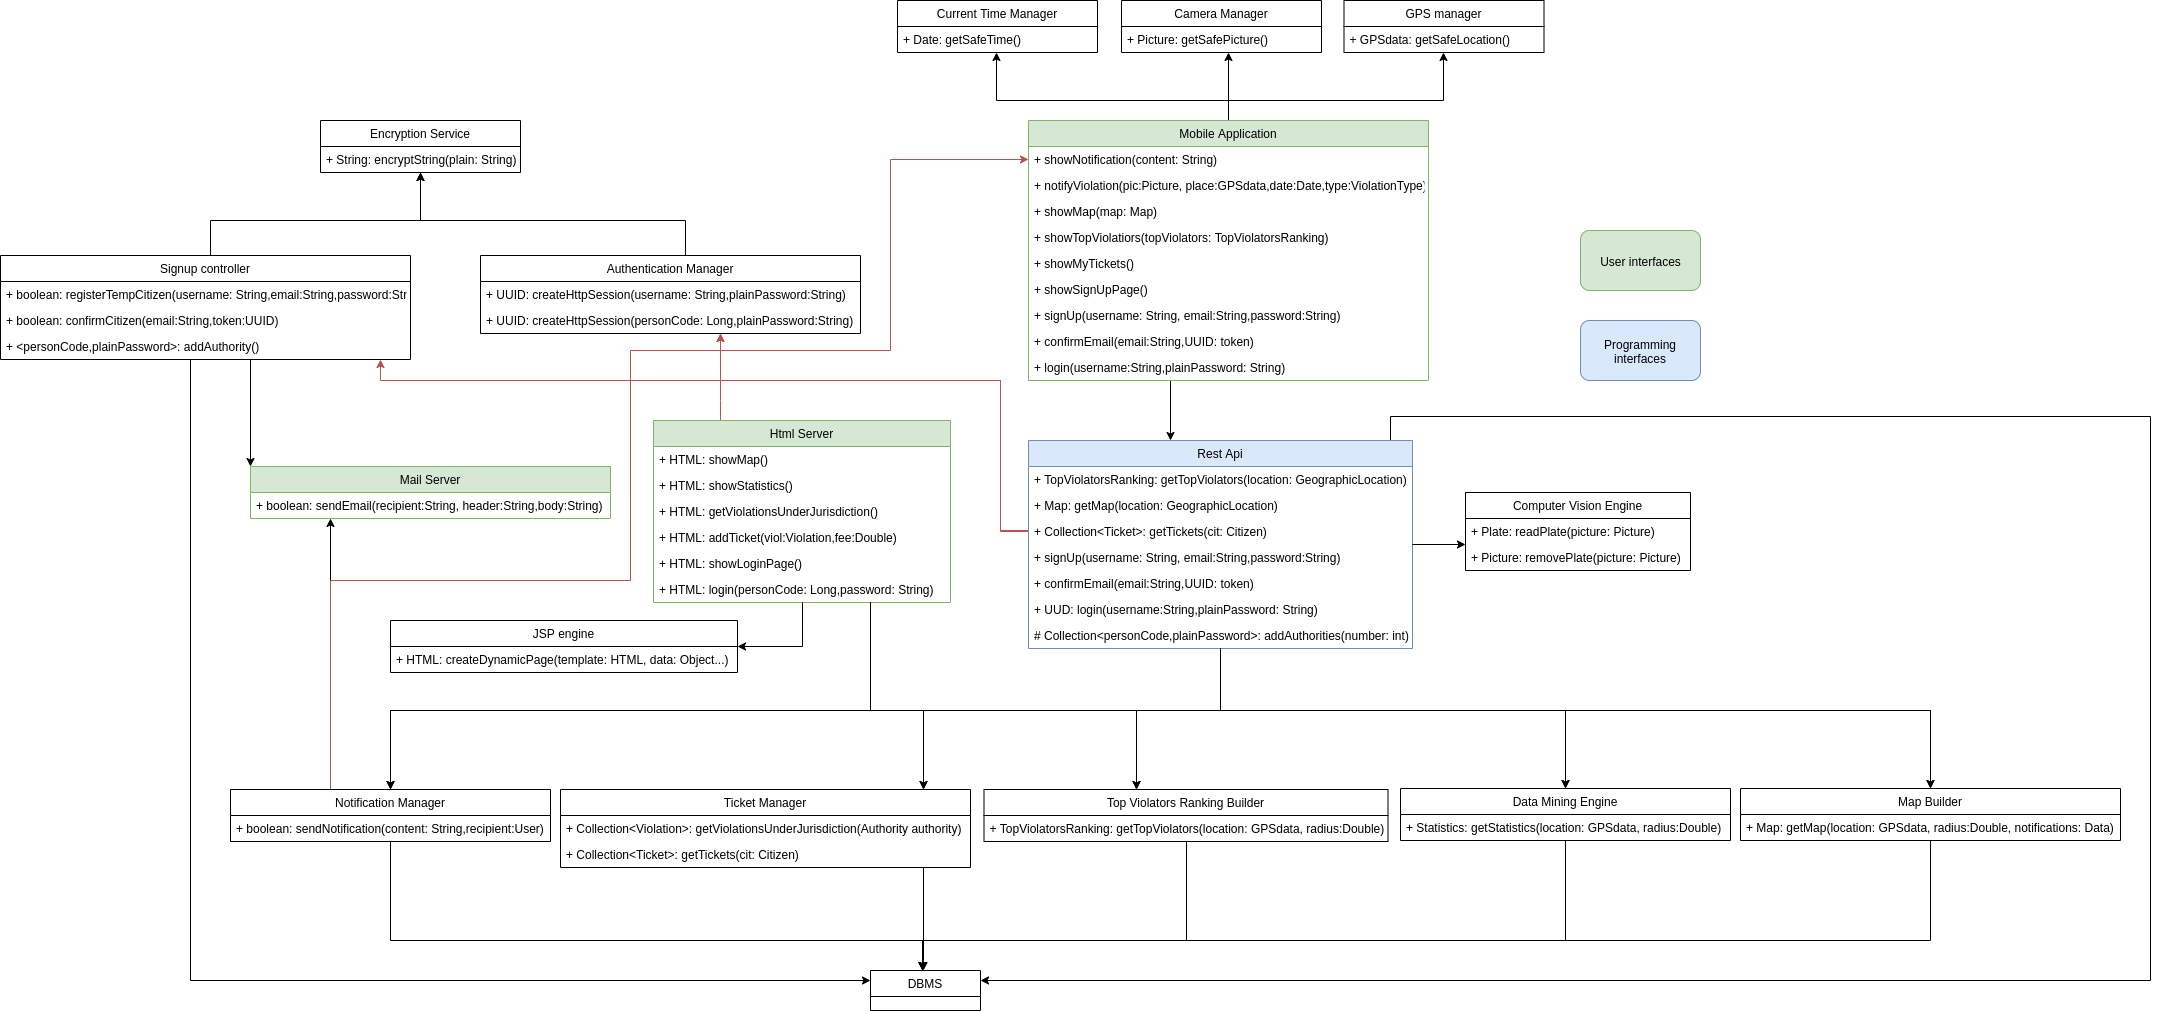
\includegraphics[width=\linewidth]{images/Interface_diagram.png}
			\caption{Component interfaces diagram}
		\end{figure}
	\subsection{Selected architectural styles and patterns} Please	explain	which	styles/patterns	you	used,	
why,	and	how
		\subsubsection{REST paradigm}
			We decided to design the system following the REpresentational State Transfer paradigm, 				in order to reduce the design complexity and improve reusability and maintainability.
			Following are stated the key concepts of REST and how they're 
			\begin{itemize}
				\item \textbf{Client-server architecture}
				\item \textbf{Stateless:} 
					The components does not store information of what they are doing. Every request comes with all the needed data to
					provide a response, or any missing data can be retrieved from the database or by transforming the already available
					data.
				\item \textbf{Cacheability:} 
					All the responses are marked as cacheable or not (if a response can be cached, overall 
					latency can be significantly reduced)
				\item \textbf{Layered:} 
					As pointed in \ref{somewhere}, the system is organized in layers and provide
					interfaces to external processes (controlled by users or automated=
				\item \textbf{Uniform interface:} 
					Uniformity of the interface is granded by exposing HTTP endpoints, which transmit resources using
					the \link{https://json.org/json-en.html}{JSON} format.
					\subitem \textbf{Resource identification:} 
						Evevry data exposed to the outside and not representational (Webpages) is 
						encoded in the JSON format. Web pages are obviously provided in 
						\link{https://en.wikipedia.org/wiki/HTML}{HTML} format, in order to be displayable by
						common web browsers.
					\subitem \textbf{Resource manipulation through representations:}
						The format of the resources can be easly modified, as are represented
						in a structured text format
					\subitem \textbf{Self-descriptive messages:}
						The JSON format names every data exchanged. The names we use are
						expressive enought to be self-descriptive
					\subitem \textbf{Hypermedia as the engine of application state:}
						Concerning the API, we provide a service broker to expose all of the
						interface mathods. With regard to the web application, it's navigable 
						using web links (see \ref{fig:homepage})
			\end{itemize}
		\subsubsection{MVC pattern}
			The \link{https://en.wikipedia.org/wiki/Model-view-controller}{Model, View, Controller} pattern is a widely 
			used pattern. Its main advantage is a significant reduction of the complexity, granted by a layered
			structure that subdivides responsibilities.
	\subsection{Other design decisions}
\newpage
\section{User Interface Design}Provide	an	overview	on	how	the	user	interface(s)	of	your	system	will	
look	like; if	you	 have	included	 this	 part	in	 the	 RASD,	you	 can	 simply	 refer	 to	what	you	 have	
already	done,	possibly,	providing	here	some	extensions	if	applicable.
	\subsection{Mobile application interface}
		\begin{figure}[H]
			\centering
			\begin{subfigure}[H]{0.49\linewidth}
				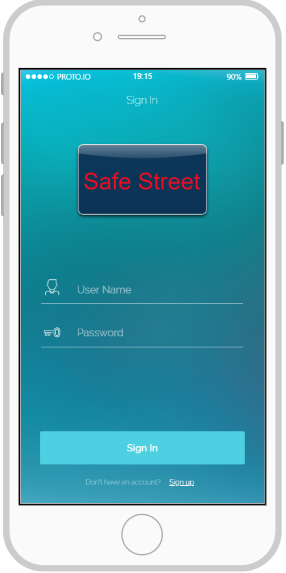
\includegraphics[width=\linewidth]{images/Sign_In.png}
				\caption{Sign in}
			\end{subfigure}	
			\begin{subfigure}[H]{0.49\linewidth}
				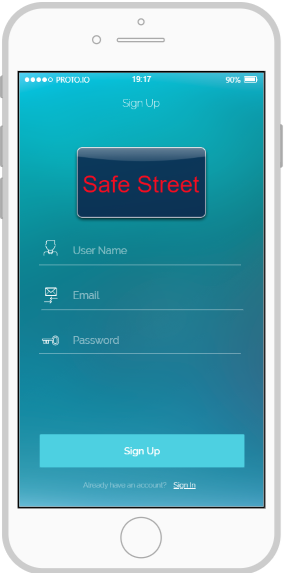
\includegraphics[width=\linewidth]{images/Sign_Up.png}
				\caption{Sign up}
			\end{subfigure}
		\end{figure}
		\begin{figure}[H]
			\begin{subfigure}[H]{0.49\linewidth}
				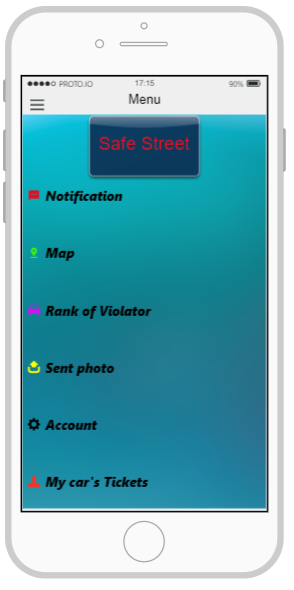
\includegraphics[width=\linewidth]{images/Menu.png}
				\caption{Menu}
			\end{subfigure}
			\begin{subfigure}[H]{0.49\linewidth}
				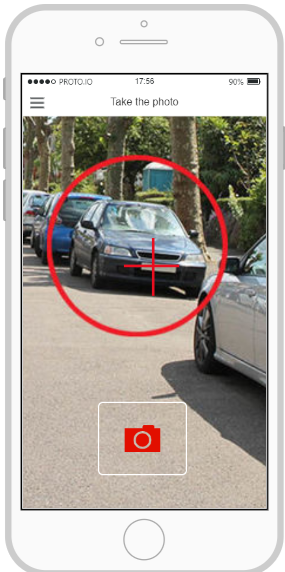
\includegraphics[width=\linewidth]{images/Camera.png}
				\caption{Camera}
			\end{subfigure}
		\end{figure}
		\begin{figure}[H]
			\begin{subfigure}[H]{0.49\linewidth}
				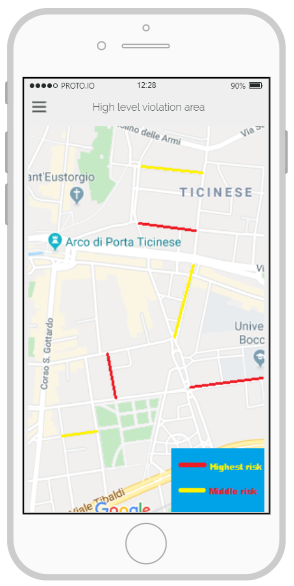
\includegraphics[width=\linewidth]{images/Maps.png}
				\caption{Map}
			\end{subfigure}
			\begin{subfigure}[H]{0.49\linewidth}
				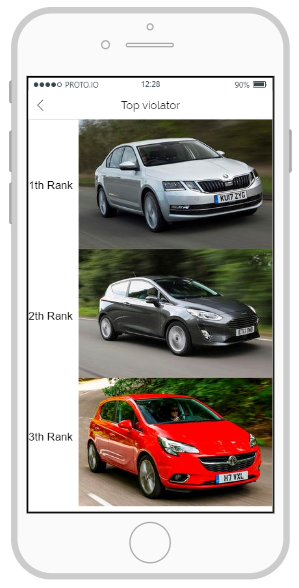
\includegraphics[width=\linewidth]{images/Top_Violators.png}
				\caption{Top Violators}
			\end{subfigure}
		\end{figure}			
	\subsection{Mobile application UX diagrams}
	\subsection{Web application interface}
		\label{fig:homepage}
		\begin{figure}[H]
			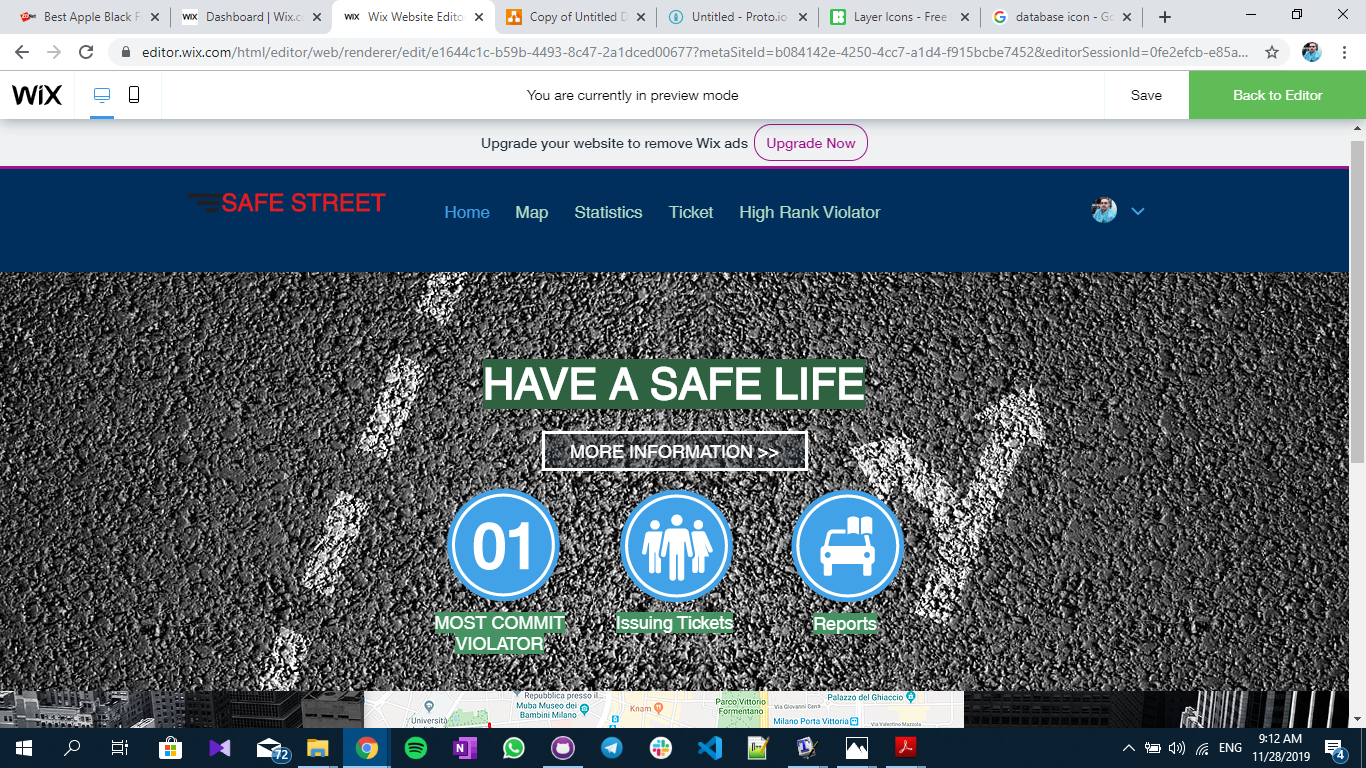
\includegraphics[width=\linewidth]{images/home.png}
			\caption{Home page}
		\end{figure}
		\begin{figure}[H]
			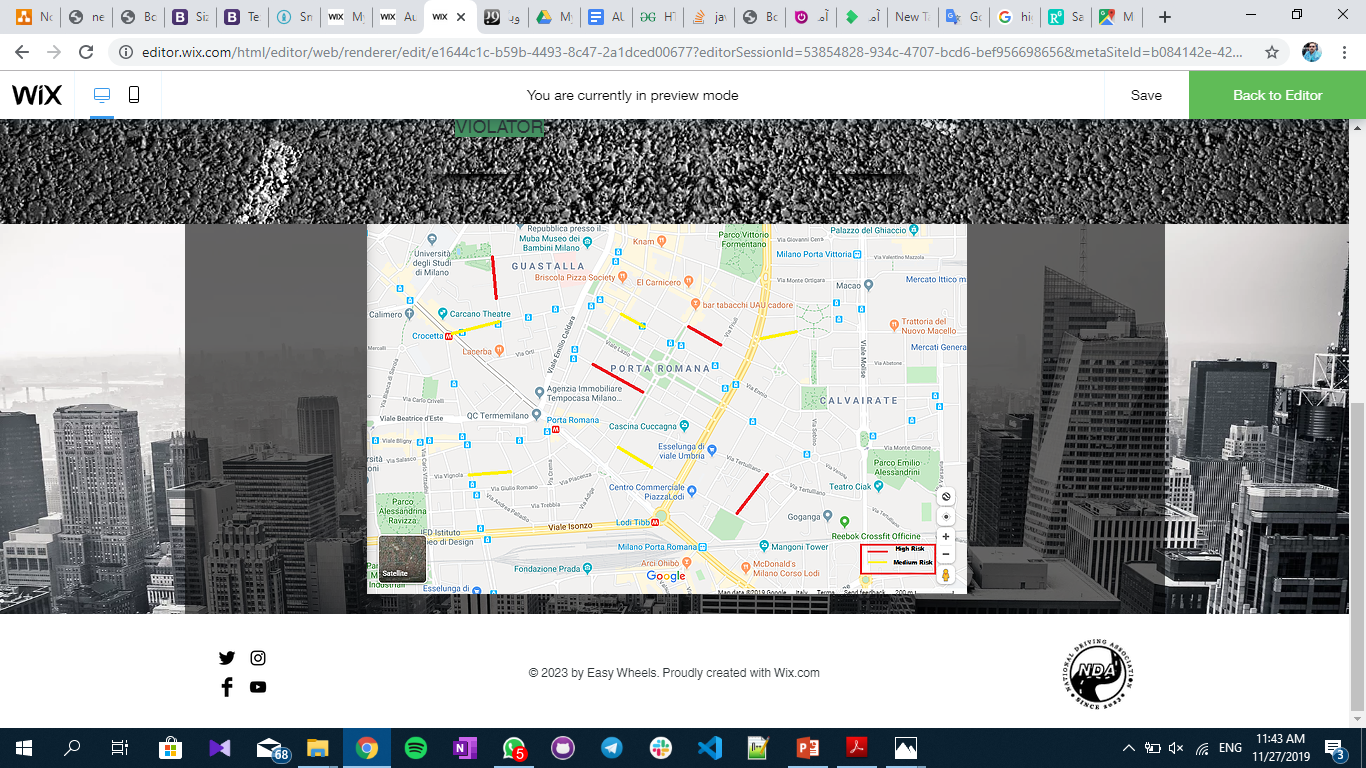
\includegraphics[width=\linewidth]{images/map.png}
			\caption{City map with risky streets marked}
		\end{figure}
		\begin{figure}[H]
			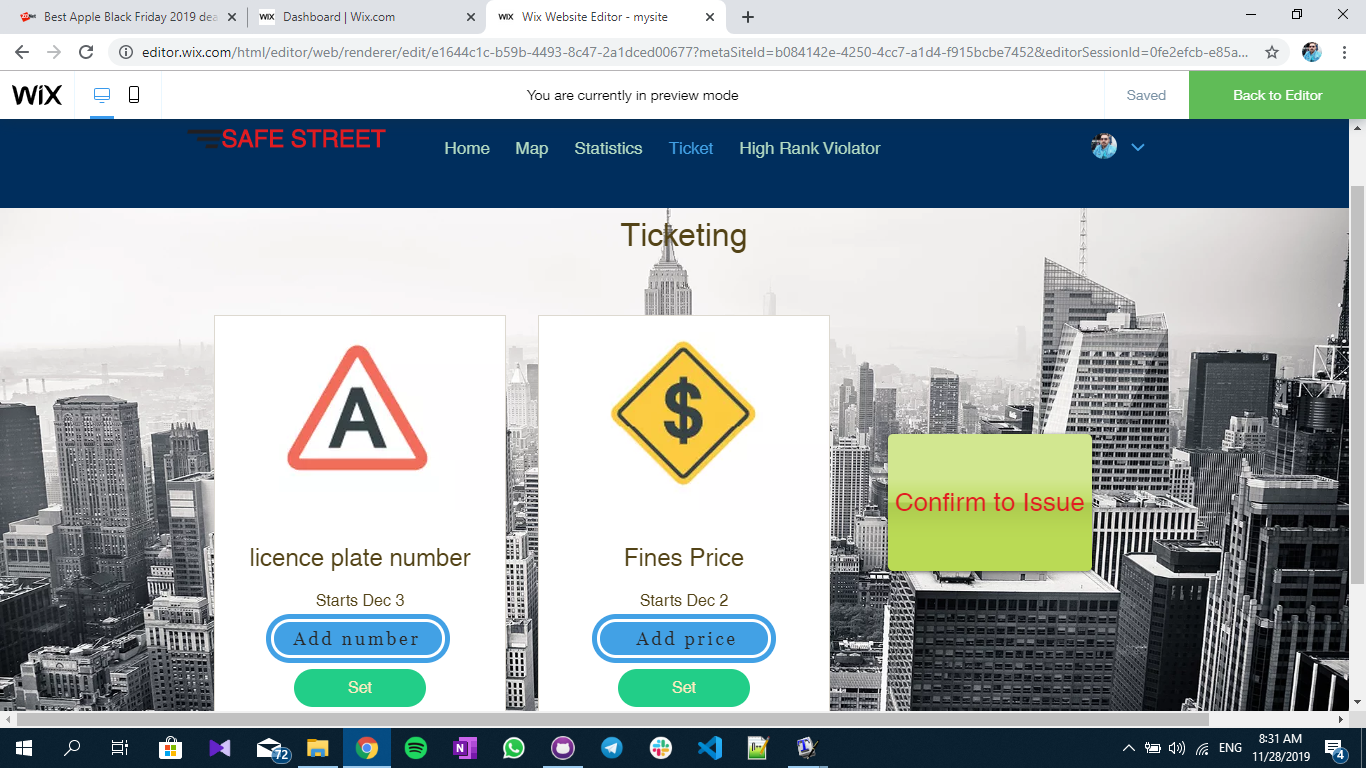
\includegraphics[width=\linewidth]{images/ticketing.png}
			\caption{Insert ticket informations}
		\end{figure}
		\begin{figure}[H]
			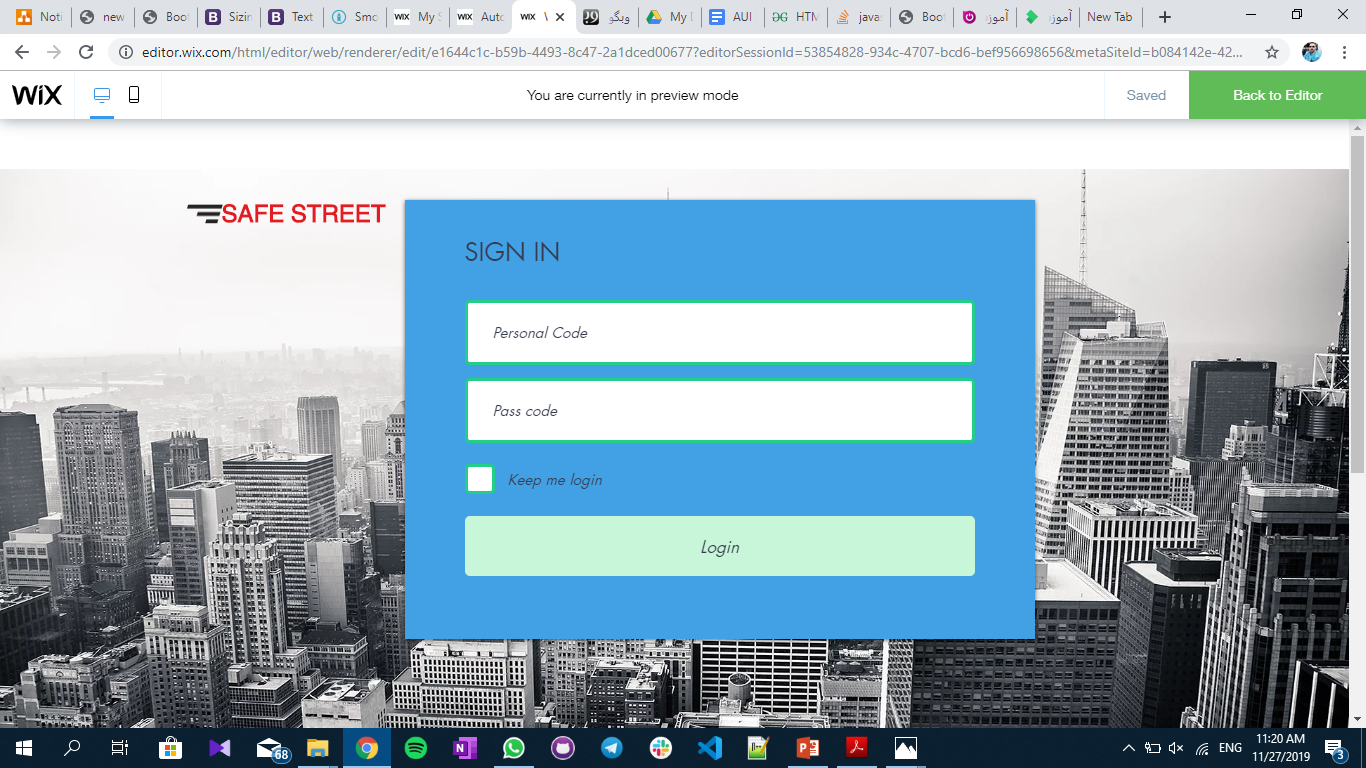
\includegraphics[width=\linewidth]{images/log in.png}
			\caption{Login screen}
		\end{figure}
	
\section{Requirement traceability}	Explain	how	the	requirements	you	have	defined	in	the	RASD	
map	to the	design	elements	that	you	have	defined	in	this	document
\section{Implementation, Integration and Test plan}	Identify 	here	the	order	in	which	you	plan	
to	implement	the	subcomponents	of	your	system	and	the	order	in	which	you	plan	to	integrate	
such	subcomponents	and	test	the	integration.	
First, each component has been prioritized for both value generated for each user-type and implementation difficulty. The results of this prioritization are displayed in the following table. For cloud-placed and bought components, the expected price and the configuration effort for the chosen implementation are both written in parenthesis. Empty cells indicate components not significant for that type of user. Finally, components fullfilled by the same service (cloud-based or bought) are not separated by horizontal lines.
\begin{table}[H]
\begin{center}
\caption{Component priorities}
\small
\begin{tabular}{|c|c|c|c|}
	\hline
	\textbf{Component}				&\textbf{Value (for citizens)}	&\textbf{Value(for authorities)}	&\textbf{Difficulty of implementation}	\\
	\hline
	Authentication Manager			&Low to Medium					&High							&Cloud (cheap,low)						\\
	Signup Controller				&Low	 to Medium					&High							&Cloud (cheap,low)						\\
	Encryption Service				&Low								&High							&Cloud (cheap,low)						\\
	\hline
	Mobile Application				&High							&								&Medium to High							\\ 
	\hline
	HTML Server						&								&High							&Buy	 (free,low)							\\
	Rest Api							&High							&								&Buy (free,low)							\\
	\hline
	Mail Server						&Low								&Low								&Cloud (cheap,low)						\\
	\hline
	JSP								&								&High							&Buy (free,low)							\\ 
	\hline
	Notification Manager				&Medium							&Medium to Low					&Low										\\ 
	\hline
	Map Builder						&High							&High							&Cloud (cheap,medium)					\\ 
	\hline
	Top Violators Ranking Builder	&Low to Medium					&								&Low										\\ 
	\hline
	Computer Vision Engine			&Medium to High					&Medium to High					&Cloud (cheap,medium to high)			\\
	\hline
	Data Mining Engine				&								&Medium to High					&High									\\ 
	\hline
	Ticket Manager					&								&High							&Low										\\
	\hline
	Camera Manager					&Medium							&High							&Medium to Low							\\ 
	\hline
	GPS Manager						&Medium							&Medium							&Medium to Low							\\ 
	\hline
	Current Time Manager				&Medium							&Medium							&Low										\\ 
	\hline
	DBMS								&High							&High							&Buy (cheap,low)							\\
	\hline
\end{tabular}
\end{center}
\end{table}
\newpage
Analyzing the table, we indentified 5 implementation phases: Prototype, Basic Logic, Authentication, Mobile Security, Extended features. Each phase is described in the following table:
\begin{table}[H]
\begin{center}
\small
\setlength\tabcolsep{0pt}
\begin{tabular}{|c|c|c|c|c|}
		\hline
		\textbf{Implementation Phase}		&\textbf{Adopted solution}					&\textbf{Covered Components}		&\textbf{Solution effort}	&\textbf{Phase Efforts}\\
		\hline
		\multirow{5}{*}{Prototype}			&Amazon S3									&DBMS							&Low				&\multirow{5}{*}{Low}			\\
											\cline{2-4}
											&\multirow{2}{*}{Tomcat Web Server}			&Rest Api						&\multirow{2}{*}{Low}&							\\
											&											&HTML Server						&				&								\\
											\cline{2-4}
											&Custom made Application						&Mobile Application				&Medium to High	&								\\
											\cline{2-4}
											&JSP											&JSP								&None			&								\\
		\hline
		\multirow{3}{*}{Basic logic}			&Amazon Rekognition							&Computer Vision Engine			&Medium to High	&\multirow{3}{*}{Medium}			\\
											\cline{2-4}
											&Google Cloud: Maps							&Map Builder						&Medium			&								\\
											\cline{2-4}
											&Custom controller							&Ticket Manager					&Low				&								\\
		\hline		
		\multirow{4}{*}{Authentication}		&\multirow{3}{*}{Amazon cognito}				&Authentication Manager			&\multirow{3}{*}{Low}&\multirow{4}{*}{Low}		\\
											&											&Signup Controller				&				&								\\
											&											&Encryption Service				&				&								\\
											\cline{2-4}
											&Amazon Simple Mail							&Mail Server						&Low				&								\\
		\hline		
		\multirow{3}{*}{Mobile Security}		&\multirow{3}{*}{Mobile Application Update}	&Camera Manager		&\multirow{3}{*}{Medium to Low}&\multirow{3}{*}{Medium to Low}\\
											&											&GPS Manager						&				&								\\
											&											&Current Time Manager			&				&								\\
		\hline
		\multirow{3}{*}{Extended features}	&\multirow{3}{*}{Custom controllers}			&Data Mining Engine				&High			&\multirow{3}{*}{Medium}			\\
											&											&Notification Manager			&Low				&								\\
											&											&Top Violators Ranking Builder	&Low				&								\\
		\hline
\end{tabular}
\end{center}
\end{table}

And in the following graph the dependencies between the phases are shown.

\begin{figure}[H]
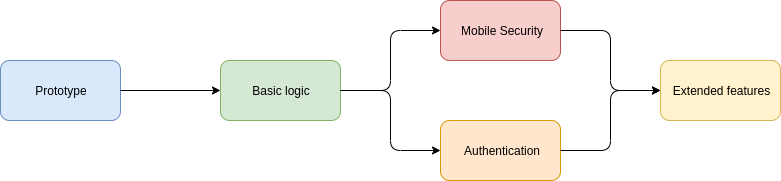
\includegraphics[width=\linewidth]{images/Implementation_phases.png}
\end{figure}

\paragraph{Unit testing}For testing, we have to assume that every outsourced solution has been tested and is perfectly working (as we can't perform unit testing on them). With regard to the Mobile Application, the Ticket Manager, the Data Mining Engine, the Notification Manager and the Top Violators Ranking Builder, a set of tests will be generated before the beginning of the coding phase in order to guide it, and to define some initial acceptance criteria. More precise tests will be developed during the coding phase, in order to test the coponent behaviour more in detail.

\paragraph{Integration testing} Into each phase, integration testing will be performed to integrate components of the same phase one with the other and with the pre-existing system (assumed to be working perfectly and already tested exhaustively). A more detailed integration and testing plan will be provided in a following version of this document.

\paragraph{Acceptance test} A set of acceptance tests will be generated at the beginning of each phase. This of acceptance tests will cover a great number of test cases, and will be usable as Regression tests as well

\section{Effort spent}In	 this	 section	you	will	include	information	about	 the	number	of	hours	each	
group	member	has	worked	for	this	document.
	\paragraph{Matteo Secco}
		\begin{itemize}
			\item 25 November: Components, toghether. 3h
			\item 27 November: Components. 3h
			\item 29 November: Deployment. 4h
			\item 5 December: Inserted images, refactor structure. 1h
			\item 7 December: Sequence diagrams. 5h
			\item 7 December: Implementation, integration and testing. 0.45h
		\end{itemize}
	\paragraph{Rahbari}
		\begin{itemize}
			\item 25 November: Components, toghether. 3h
			\item 27.28 November: Interface. 3h
		\end{itemize}
\section{References}

\end{document}